\chapter{Introduction}

% 1) ZACIATOK O PARALELIZACII VSEOBECNE
These days, we are increasingly encountering parallel programs.
A dozen programs that have been written in a typical way for single-core systems cannot take advantage of the presence of computers with multiple cores.
When we wanted to speed up problem-solving, we wanted to create something that would eliminate our time on calculations.
Thus, we invented the computer, which at the beginning knew relatively nothing to do.
However, after a few years, all this changed, and the computer solved problems that took a person many days.
Today, we live when computers have significantly improved execution time by solving different problems using parallelism.

% 2) Úvod do problematiky + motviacia pre tuto diplomku
In recent years, many companies have adopted Kubernetes and the microservices architecture it enables.
This technology was opened up many new possibilities not just for large companies, but also for small software developers.
Kubernetes is a container-orchestration system and recently a new concept has emerged around how to orchestrate the containers more efficiently \---\ the Operator pattern.
One such operator is developed and maintained under an open-source project called Strimzi.
The Strimzi project gathers together several tools, which take care of the deployment of Apache Kafka on Kubernetes.
Since Kafka is a complex, horizontally scalable, distributed system, you can imagine that its installation is a relatively complex action.
Therefore, one of the biggest challenges of using Kubernetes is how to effectively and quickly test projects such as Kafka and Strimzi and at the same time verify integration with other similar products.
The resources needed by Kubernetes are much more demanding compared to the deployment of Kafka on virtual machines or typical container instances.
To tackle this problem, we adopt the principles of parallel execution and created a mechanism within Strimzi system tests, which runs tests in parallel against only a single Kubernetes cluster.
Furthermore, we proposed a brand-new architecture for the end-to-end tests.
The improvements aim at \textit{scalability} and \textit{reduction of execution time}.
Through several experiments, this paper shows that proposed mechanism with different configurations of the Kubernetes cluster (including \textit{number of Kubernetes nodes}, \textit{number of tests and suites executed in parallel}) significantly accelerated execution of the tests.

% Related work
Related work focuses on improving the overall verification time of a Strimzi product.
For a long time and many releases of Strimzi, testing using a sequential computational model has been extremely slow.
At the same time, the product contains about 15 of the most critical possible combinations of product deployment, each of which lasts over sixty hours.
This sequential computational model is not a recommended candidate for verifying such a large number of deployments.
An attentive reader could see the entire test time approaching 1000 hours, approximately one and a half months.
Nevertheless, as part of this effort for coarse-grained parallelism in performing multiple product deployments, it partially accelerated the overall computation.
However, this approach is not horizontally scalable due to our cloud services that provide resources (i.e., bare metals, virtual machines, containers).
Therefore, we got to the last opportunity to improve the computation using the vertical scalability of the resources (i.e., memory, central processing units) that the cloud services offer us.
This information motivated us to design and implement a mechanism of fine-grained parallelism in our test framework.
Figure \ref{00:fig:evolution} shows the overall evolution of our test framework and summarises the previously mentioned sentences.

\begin{figure}[!ht]
    \centering
    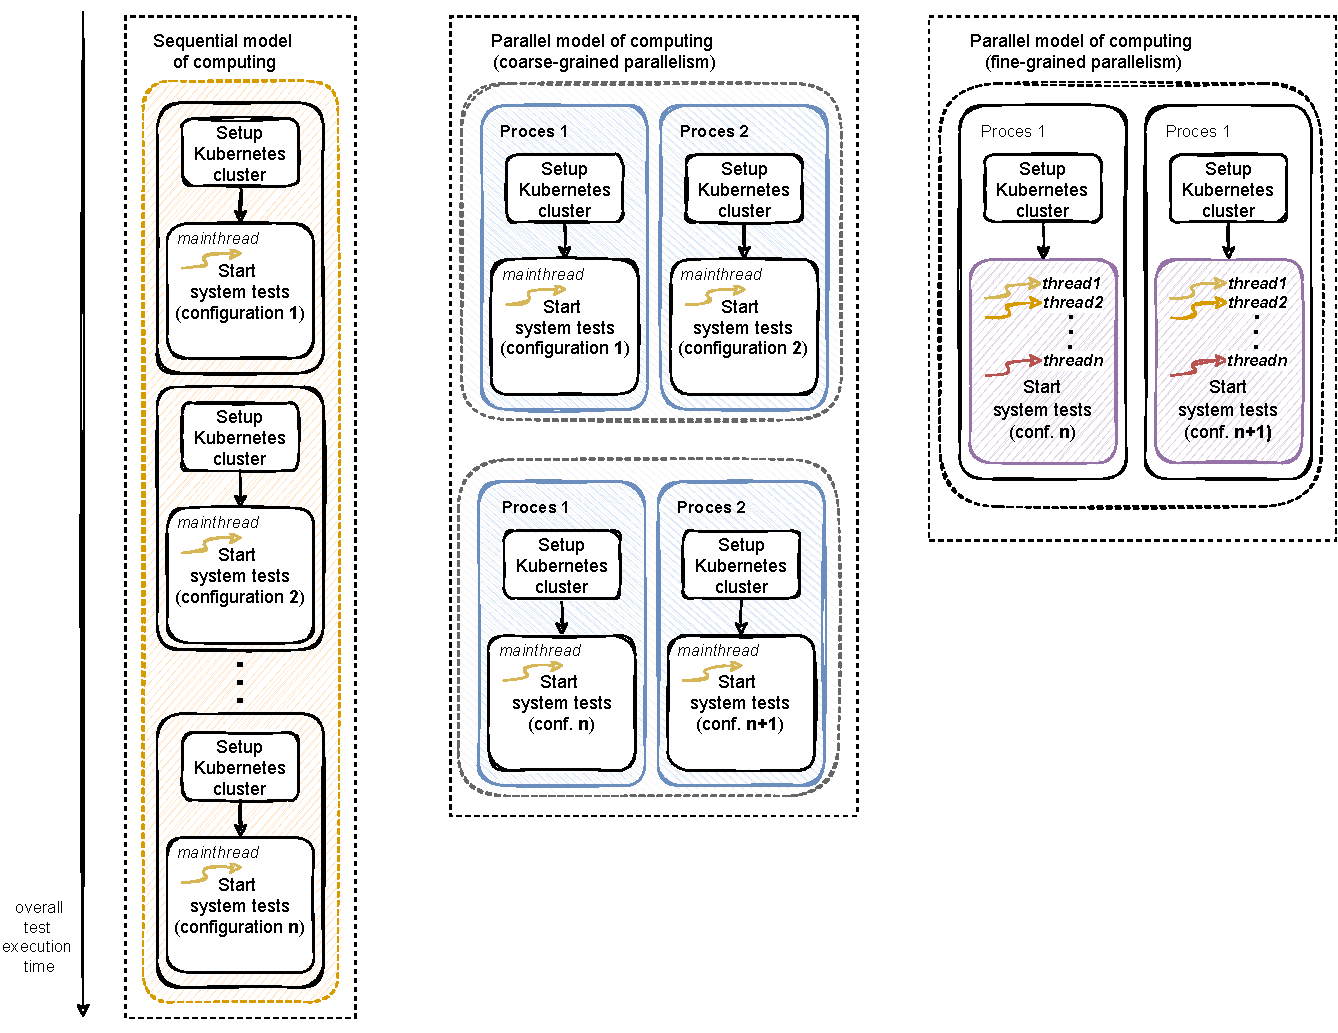
\includegraphics[scale=0.7]{obrazky-figures/01-intro/00-intro-better-one}
    \label{00:fig:evolution}
    \caption{Evolution of our test framework execution}
\end{figure}

% 4) Prínosy tejto práce
\subsubsection*{Acquisition of this work}

This work deals with the parallelisation of Kubernetes Strimzi system tests.
The author contributed the given code to the open-sourced project Strimzi available on Github\footnote{\textbf{Strimzi Github repository} \ ---
\url{https://github.com/strimzi/strimzi-kafka-operator}}, which also makes it possible to inspire other \emph{kube-native} products.
The comprehensive benefit of this work is the significant acceleration of the verification process.

\subsubsection*{The structure of the diploma thesis}

In Chapter \ref{02:chapter:title}, the reader will learn the theoretical background to understand the overall thesis (i.e., Kubernetes (\ref{01:sec:title}), Apache Kafka (\ref{02:sec:title}), Strimzi (\ref{03:title})).
In Chapter \ref{03:chapter:title}, we explain the fundamental concepts of parallelism (i.e., Amdahl's law (\ref{04:amdalhlaw}), Shared memory ()\ref{04:sharedmemory}), Process and Thread (\ref{04:processesandthreads}), Synchronisation (\ref{04:synchronization}).
Chapter \ref{04:chapter:title} presents bottlenecks in the current approach of testing the Strimzi product and proposes a brand-new computational architecture that solves many issues.
In Chapter \ref{05:chapter:title}, we describe the implementation of the proposed architecture.
Chapter \ref{06:chapter:title} presents many experiments with deep analysis on the thesis implementation.
Finally, in Chapters \ref{07:chapter:title},\ref{08:chapter:title}, we conclude the entire diploma with the knowledge that has been acquired, and at the same time, we discuss possible directions for possible future work.